\subsection*{Trama de Supervisión}
Las tramas con el formato de supervisión (\texttt{S}) son usadas para llevar a cabo el control de flujo y el control de errores. Estas confirman la recepción de las tramas \texttt{I}. No se permite el transporte de información en las tramas de supervisión.
\\${ }$\\
Si los primeros dos bits del campo de control son \texttt{10}, esto significa que la trama es una trama \texttt{S}, Los ultimos 3 bits llamados $N_r$ corresponden al número de reconocimiento o al número de reconocimiento negativo según el tipo de trama \texttt{S}. El codigo llamado de 2 bits se utiliza para definir el tipo de trama:
\begin{itemize}
\item \texttt{RR} (Receive Ready, Receptor Preparado) \texttt{S=00} 

Se utiliza para indicar la disponibilidad de recepción de tramas y confirmación de tramas con el subcampo $N_r$. Una trama \texttt{RR} es enviada por una estación primaria o secundaria para confirmar que ha recibido correctamente las tramas hasta $N_r -1$ para indicar que ya esta listo para recibir las tramas $N_r$. La trama \texttt{RR} sondea (polling) una línea multipunto o una línea punto a punto. La estación primaria envía a la secundaria y le solicita que le envíe alguna trama de datos pendiente, es decir la primera trama que contenga la solicitada $N_s$.

\item \texttt{RNR} (Receive Not Ready, Receptor no Preparado) \texttt{S=01} 

Esta trama envía tanto una estación secundaria como primaria para indicar que está temporalmente ocupada y que no puede aceptar tramas de información. El número de secuencia $N_r$ es el número de la trama esperada aproximadamente después que la condición de ocupación termine y puede usarse para confirmar que las tramas $N_r$ se recibieron correctamente.

\item \texttt{REJ} (Reject, Rechazo Simple) \texttt{S=10} 

Utilizado para confirmar la recepción de tramas anteriores $N_r$ y solicitar posteriores. Esta condición se libera cuando las tramas solicitadas o un comando de cambio de modo fueron correctamente recibidos.

\item \texttt{SREJ} (Selective Reject, Rechazo Selectivo) \texttt{S=11} 

Confirma la recepción de las tramas anteriores a la $N_r$ y solicita la retransmisión de la $N_r$. Una trama \texttt{SREJ} debe ser transmitida por cada trama errónea, pero con la siguiente limitación. Solo puede haber una trama \texttt{SREJ} pendiente, el envío de una segunda trama \texttt{SREJ} contradice la primera puesto que todas las tramas \texttt{I} con $N_s$.

\end{itemize}

\subsection*{Ventana Deslizante}
Es un mecanismo dirigido al control de flujo de datos que existe entre un emisor y un receptor pertenecientes a una red. Es bidireccional. La ventana deslizante es un dispositivo de control de flujo, es decir, el control de flujo se lleva a cabo mediante el intercambio específico de caracteres o tramas de control con lo que el receptor indica al emisor cual es su estado de disponibilidad para recibir datos. \\${ }$\\
Es necesario para no inundar el receptor con envíos de tramas de datos, que el receptor al recibir datos sean procesados si no lo realiza a la misma velocidad que el transmisor la envía, se verá saturado y parte se puede perder.
\subsubsection*{Funcionamiento}
Permite al emisor transmitir múltiples segmentos de información antes de comenzar la espera para que el receptor le confirme la recepción de los segmentos, tal confirmación se llama validación y consiste en el envío de mensajes denominados \texttt{ACK} del receptor al emisor. La validación se realiza desde el receptor al emisor y contiene el número de la siguiente trama que espera recibir el receptor, o el de la última trama trama recibida con éxito. $\texttt{ACK}_n$ (número de tramas indicada). Con esto el emisor es capaz de distinguir el número de los envíos realizados con éxito, los envíos pedidos y la que se esperan.
\subsubsection*{Elementos}
\begin{itemize}
\item \textbf{Tranmisión:} Permite el emisor transmitir múltiples paquetes de información, sin recibir confirmación de la recepción correcta de la misma.
\item \textbf{Validación:} Cuando llega un paquete al receptor, este envía un \texttt{ACK} al emisor. \texttt{ACK}: del paquete recibido indicando cual es el paquete. \\${ }$\\
Se lleva a cabo de la siguiente manera:
\begin{itemize}
\item \textbf{Piggybacking:} Técnica de retardar temporalmente los \texttt{ACK} para que puedan viajar en el siguiente paquete de datos.
\item Los paquetes enviados pero no validados se denominan Unacknowledge.
\item Los paquetes unacknowledge estan limitados por la ventana.
\end{itemize}
\item El protocolo no espera a la validación por paquete, esto hace que exista una contínua transmision de información.
\item \textbf{Buffer:} guarda un buffer todos los paquetes enviados y no validarlos si es que necesitan ser retransmitidos. Este debe ser igual o mayor al tamaño de la ventana y solo es eliminado si llega un \texttt{ACK}, así se desliza la ventana.
\item \textbf{Temporizador:} El buffer asigna un temporizador a cada uno de los paquetes transmitidos. El temporizador limita el tiempo de esperar para la validación de cada paquete. Si se acaba el tiempo sin éxito, se reenvía.
\item \textbf{Ventana de Recepción:} Se ordenan siguiendo una lista secuencial. Los almacena en un buffer hasta que termine la transmisión.
\end{itemize}

%\begin{figure}[H]
%\centering
%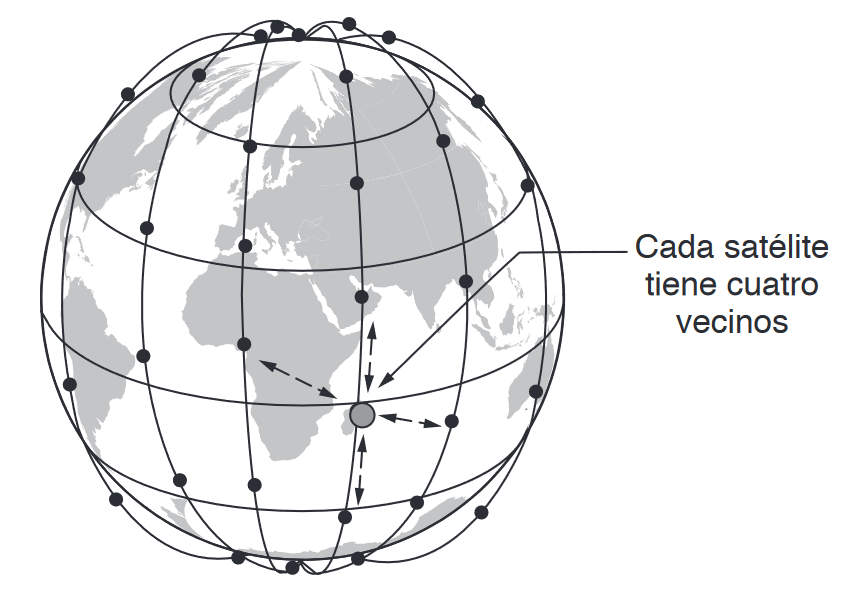
\includegraphics[page=1,scale=0.7]{SATELITES2.png}
%\caption{Satélites Iridium \textit{(Redes de Computadoras, Tanenbaum 4ta Edición, Pagina 105)}}
%\end{figure}

%\begin{figure}[H]
%\centering
%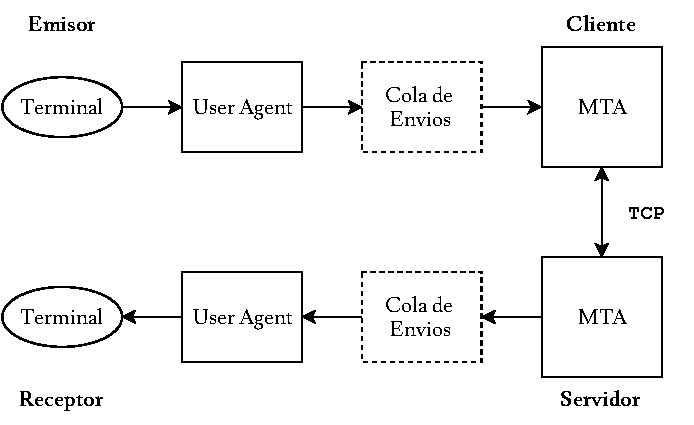
\includegraphics[page=1,scale=0.7]{SMTP.pdf}
%\caption{Esquema de funcionamiento de SMTP}
%\end{figure}
